\documentclass[11pt]{article}
\usepackage[a4paper, total={17cm, 25cm}]{geometry}

\usepackage{graphicx}
\usepackage{mathtools}
\usepackage{listings}
\usepackage{color}
\definecolor{dkgreen}{rgb}{0,0.6,0}
\definecolor{gray}{rgb}{0.5,0.5,0.5}
\definecolor{mauve}{rgb}{0.58,0,0.82}
\lstset{
  language=Java,
  aboveskip=1mm,
  belowskip=1mm,
  showstringspaces=false,
  columns=flexible,
  basicstyle={\small\ttfamily},
  numbers=none,
  numberstyle=\tiny\color{gray},
  keywordstyle=\color{blue},
  commentstyle=\color{dkgreen},
  stringstyle=\color{mauve},
  breaklines=true,
  breakatwhitespace=true,
  tabsize=3
}

\begin{document}
\thispagestyle{empty}

\begin{center}
 
\hspace{-8.5cm}{
\begin{minipage}[]{\linewidth}% to keep image and caption on one page
\center 
\includegraphics[scale=0.3]{bqlogo.png}
\end{minipage}
\hspace{3.5cm}Alvaro Ferr\'an Cifuentes
}

\vspace{1.75cm}
\textsc{\Huge Hardware Calculations}

\end{center}

\bigskip \flushleft

This document's purpose is to explain the current sensor calculations and the temperature sensor's equation.

\section*{Current Sensor}
Since the board uses a TI DRV8837 motor driver with a 1.8A maximum current, that is the range the LPC11U24's ADC should work in.\\[0.25cm]

To measure the current used by the motor a  10m$\Omega$ shunt resistor (R5) is added between the driver's GND pin and the ground plane. From Ohm's Law, for every 1000mA through the resistor there is a 10mV voltage drop, which means an 18mV range.\\[0.25cm]

The ADC works between 0 and 3.3V and has a 10-bit resolution, or a 3.23mV/step resolution. With this setup only the first 6 steps of the 1024 would be meaningful, which is a meager 0.6\% of the ADC's scale. 

\vspace{0.5cm}
\begin{minipage}[]{\linewidth}% to keep image and caption on one page
\center 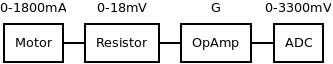
\includegraphics[width=8cm]{./Dia/Diagram1.png}
\end{minipage}
\\[0.5cm]

To use the ADC's full scale the resistor's voltage range must be transformed to that of the ADC, which is done by multiplying by the operational amplifier's gain G.

\center $G=\frac{3300}{18}=183.33$

\flushleft To get such gain the OpAmp is configured as a non-inverting amplifier, as seen in the following image:

\vspace{0.5cm}
\begin{minipage}[]{\linewidth}% to keep image and caption on one page
\center 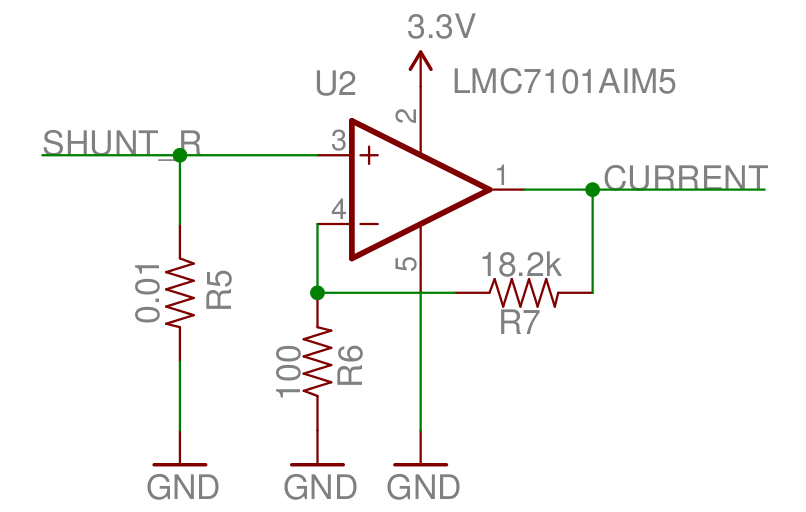
\includegraphics[width=8cm]{OpAmp.png}
\end{minipage}
\\[0.5cm]

\center $G=1+\frac{R7}{R6}$
\center $G=1+\frac{18.2k}{100}$
\\[0.4cm]

The ADC will now use its full scale to read the current, with a theoretical resolution of 1.76mA/step.

\newpage \thispagestyle{empty}
\bigskip \flushleft


\section*{Temperature Sensor}
The board includes a TMP36 temperature sensor from Analog Devices. From its datasheet:

\vspace{0.5cm}
\begin{minipage}[]{\linewidth}% to keep image and caption on one page
\center 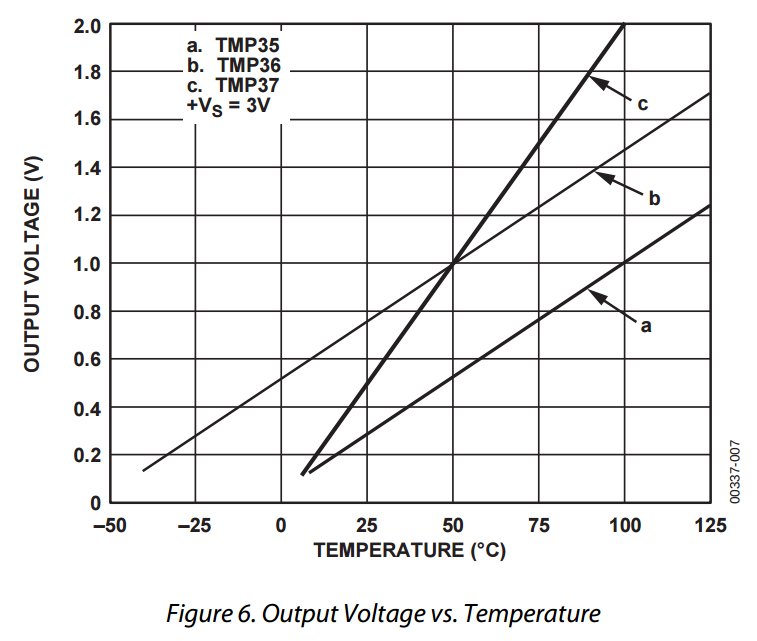
\includegraphics[width=10cm]{tmp36.png}
\end{minipage}
\\[0.5cm]

and TMP36 Output Voltage when T=25$^\circ$C is 750mV. Knowing this, the temperature equation is calculated:

\center $V(mV)=m\cdot T(^\circ C)+p$
\center $m=\frac{1000-750}{50-25}=10$
\center $p=V-m\cdot T=750-10\cdot25=500$
\center $V(mV)=10\cdot T(^\circ C)+500$
\\[1cm]
\center $\rightarrow T(^\circ C)= (V(mV)-500)/10$


\end{document}
